\documentclass[handout,11pt]{beamer}
\usetheme{Madrid}
\usepackage[utf8]{inputenc}

\usepackage[English]{babel}

\usepackage{amsmath}
\usepackage{amsfonts}
\usepackage{amssymb}
\usepackage{graphicx}
\DeclareMathOperator {\argmin}{argmin}

\author{Vansh Kapoor \& Pranava Singhal}
\title{Raptor Codes}

% Informe o seu email de contato no comando a seguir
% Por exemplo, alcebiades.col@ufes.br
\newcommand{\email}{email}
%\setbeamercovered{transparent} 
\setbeamertemplate{navigation symbols}{} 
%\logo{} 
\institute[]{EE605 Course Project \\ 
Guide: Prof. Nikhil Karamchandani} 

\date{November 24, 2022}

%\subject{}

% ---------------------------------------------------------
% Selecione um estilo de referência
\bibliographystyle{apalike}

%\bibliographystyle{abbrv}
%\setbeamertemplate{bibliography item}{\insertbiblabel}
% ---------------------------------------------------------

% ---------------------------------------------------------
% Incluir os slides nos quais as referências foram citadas
%\usepackage[brazilian,hyperpageref]{backref}

%\renewcommand{\backrefpagesname}{Citado na(s) página(s):~}
%\renewcommand{\backref}{}
%\renewcommand*{\backrefalt}[4]{
%	\ifcase #1 %
%		Nenhuma citação no texto.%
%	\or
%		Citado na página #2.%
%	\else
%		Citado #1 vezes nas páginas #2.%
%	\fi}%
% ---------------------------------------------------------

\begin{document}

\begin{frame}
\titlepage
\end{frame}

\begin{frame}{Summary}
\tableofcontents 
\end{frame}

\section{Motivation}
\begin{frame}{Motivation}
The Internet is a Binary Erasure Channel\\

Protocols like TCP/IP \& UDP are used for communication

\end{frame}

\begin{frame}{TCP/IP Shortcomings\\Idle Times}
\begin{figure}
    \centering
    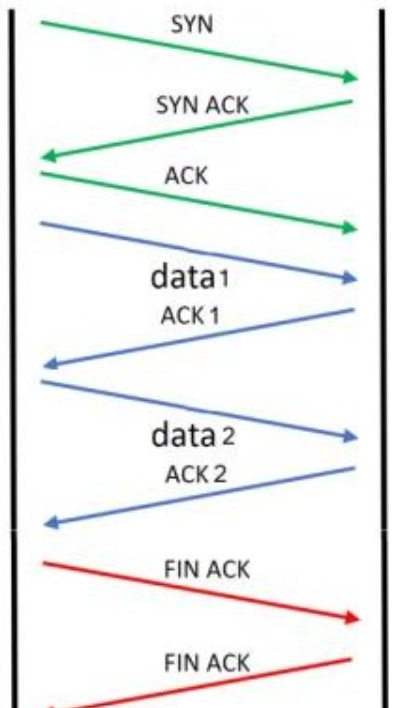
\includegraphics[scale = 0.4]{images/tcpip.PNG}
    \caption{sender waits for ACK (acknowledgement)}
    \label{fig:tcpip}
\end{figure}
\end{frame}

\subsection{Shortcomings of TCP/IP}
\begin{frame}{TCP/IP Shortcomings\\Point to Multi-Point}
\begin{figure}
    \centering
    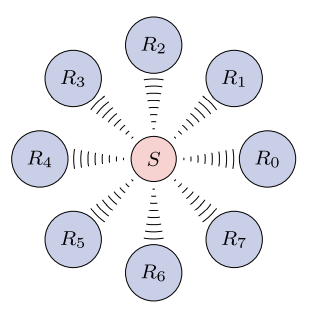
\includegraphics[scale = 0.9]{images/P2MP.png}
    \caption{Channel Usage $\mathtt{\sim}$ O(\# receivers)}
    \label{fig:my_label}
\end{figure}
\end{frame}

\begin{frame}{TCP/IP Shortcomings\\Multi-Point to Point}

\begin{figure}
    \centering
    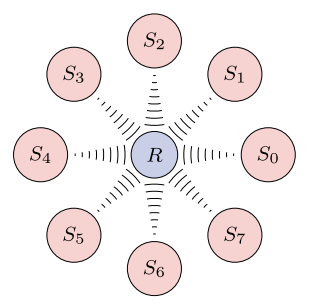
\includegraphics[scale =  0.9]{images/MP2P.png}
    \caption{Unsynchronised transmitters create redundancy}
    \label{fig:my_label}
\end{figure}

\end{frame}

\begin{frame}{TCP/IP Shortcomings\\Multi-Point to Multi-Point}

\begin{figure}
    \centering
    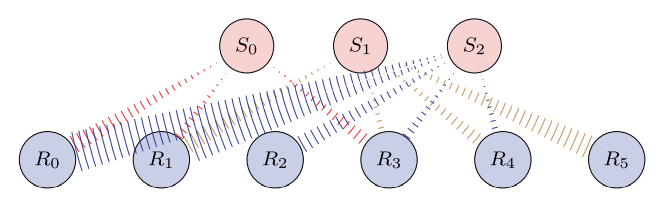
\includegraphics[scale = 0.8]{images/MP2MP.png}
    \caption{Transient nodes - Peer to Peer Networks}
    \label{fig:my_label}
\end{figure}

\end{frame}

\subsection{UDP}
\begin{frame}{UDP}
Advantage: Maximum transmission rate\\
Disadvantage: Unreliable
\end{frame}

\subsection{Conventional Error Coding}
\begin{frame}{UDP with Conventional Error Coding}
Can handle erasures but leads to increased overhead
\end{frame}

\section{Fountain Codes}
\subsection{Design Requirements}
\begin{frame}{Designing a New Class of Codes}
Design Objectives
\begin{enumerate}
    \item Unlimited transmission rate - limited only by encoding rate
    \pause
    \item An infinite stream of output symbols must be generated
    \pause
    \item All symbols must be independently generated
    \pause
    \item Any $k(1+\epsilon)$ received symbols should be enough to recover the original $k$ message symbols
    \pause
    \item Encoding and decoding cost $\mathtt{\sim}$ O(1) = constant number of operations per input message symbol 
\end{enumerate}

\end{frame}

\begin{frame}{Fountain Codes}
\begin{itemize}

\item $k$ message symbols $x_1, x_2, ..., x_k$

\item Infinite stream of output symbols $z_1, z_2, z_3, ...$
\pause 

\item Each $z_i$ is the XOR of some message symbols

\item The subset of message symbols to be XOR-ed is sampled from a distribution $\mathnormal{D}$
\pause

\item For now, assume that this combination is known to the receiver for each output symbol it receives
\end{itemize}

\end{frame}

\subsection{LT Codes}
\begin{frame}{LT Codes}
LT codes are a particular class of Fountain codes designed as follows
\vspace{1cm}
\pause

Let $\Omega_d$ denote the probability of choosing a given value $d$ $\in$ $\{1,2,..k\}$. The distribution generator polynomial is given by 
$\Omega\left (x \right)=\sum_{d=0}^{k}\Omega_d x^d$
\pause

\vspace{1cm}
$\Omega\left (x \right)$ induces a distribution on $F_{2}^{k}$ such that for any v $\in$  $F_{2}^{k}$ of weight d the probability of v is  $\Omega_d/{k \choose d}$
\pause

\vspace{1cm}
Ex: Uniform distribution on $F_{2}^{k}$ is given by $\Omega\left (x \right) = \frac{1}{2^k} \left (1+x)^k\right$

\end{frame}

\begin{frame}{Code Performance Metrics}
\begin{block}{Definitions}
\begin{itemize}

\item Encoding Cost: Expected number of operations needed to generate a single output symbol
\pause

\item Decoding Cost: Expected number of operations needed to recover a single input symbol
\pause

\item Overhead: $\epsilon =\frac{n-k}{k} \Rightarrow n=k(1+\epsilon)$ 
\pause

\item Reliable Decoding: the error probability is at most $1/k^u$ for some positive constant $u$

\end{itemize}
\end{block}
\end{frame}


\begin{frame}{Encoding Cost (1)}
\begin{block}{Proposition 1}
If an LT-code with k-input symbols possesses a reliable decoding algorithm, then there is a constant c such that the graph associated to the decoder has at least $ck\log\left (k \right)$ edges
\end{block}
\pause

\begin{block}{Proof}
Let d denote the degree of a particular output node whose distribution is given by $\Omega_d$.
\pause
The probability that a given input node is not its neighbour is

$P\left (k \right) =\sum_{d=1}^{k}\Omega_d \cdot \left (1 - d/k \right)=1-a/k$, 
where a is the expected degree of the output node and is given by $\Omega^{'}\left(1 \right)$. 
\pause
Thus the probability that the given input node is connected to none of the n output symbols is $(1-a/k)^{n}$.
\pause
We know that $-ln\left (1-x \right)= x + \frac{x^2}{2} + \frac{x^3}{3}...\le x/(1-x)$ (for $x < 1$)

\end{block}
\end{frame}

\begin{frame}{Encoding Cost (2)}
\begin{block}{Proof Continued}
Thus we get -$ln\left (1-a/k \right)\le(a/k)(1-a/k)$

$\Rightarrow (1-a/k)^n\ge e^{-\alpha/(1-\alpha/n)}$

Since the decoder is reliable
\pause
$\Rightarrow (1-a/k)^n \le 1/k^u$

$\Rightarrow e^{-\alpha/(1-\alpha/n)}\le 1/k^u$, where $\alpha$ = $an/k$
(the expected number of edges per input symbol)

\begin{align*}

\Rightarrow \alpha & \ge\ln\left(k\right)\frac{u}{(1+u\ ln\left(k\right)/n)}\\
 & \ge ln\left(k\right)\frac{u}{(1+u\ ln\left(k\right)/k)}\\
 & \ge ln\left(k\right)\frac{u}{(1+u\ ln\left(3\right)/3)}\\
\Rightarrow \alpha & = c \log\left(k\right)
\end{align*}
This implies the encoding cost is O($\log k)$
\end{block}
\end{frame}

\section{Decoding Algorithms}
\begin{frame}{Decoding Algorithms (1)}
Maximum Likelihood Decoding
\begin{itemize}
\item In the case of an erasure channel ML decoding is nothing but Gaussian Elimination
\pause

\item Each output symbol is a linear combination of a certain number of input symbols
\pause

\item View it as solving n linear equations in k unknowns

\item Thus the decoding cost of of this algorithm is O($nk$) (because Gaussian elimination can be performed in O($nk^2$) operations)
\end{itemize}
\pause

\begin{block}{Fact}
A Random LT-code with k input symbols has encoding cost k/2, and ML decoding is a reliable decoding algorithm for this code with overhead O($\log{k}/k$)
\end{block}
\end{frame}

\begin{frame}{Decoding Algorithms (2)}
ML Decoding has O($k^2$) complexity. We want a more efficient decoder

Belief Propagation Decoding\\

Imagine the graph associated to the decoder. It performs the following steps until either no output symbols of degree 1 are present or all input symbols have been recovered.

\begin{itemize}
\item Step 1: Identify all output symbols of degree 1
\pause
\item Step 2: If no output symbols of degree 1 are present are not all input symbols have been recovered then report a decoding failure else the value of the output symbol(of degree 1) gives the value of the input symbol
\pause
\item Step 3: After decoding the input symbol add its value to all the neighbouring output symbols(Basically we are eliminating all the edges from the recovered input node)
\pause
\item Step 4: Repeat the process until all the input symbols are recovered or a decoding failure is received
\end{itemize}

Decoding Cost of BP decoder is O($k$)

\end{frame}

\begin{frame}{Decoding Algorithms (3)}
Random LT-codes fail miserably with BP decoder. Can you guess why?
\pause
We need to change the design of $\Omega(x)$

The Soliton Distribution is given by

$\Omega\left (x \right)=\frac{x}{k} + \sum_{k\ge d\ge2}^{\infty}\frac{x^d}{d(d-1)}$ 

\pause

A slight variation of Soliton Distribution by Luby is an excellent distribution for BP decoding and reliable overhead of O($\log^2\left (x \right)/\sqrt k)$
\end{frame}
\section{Raptor Codes}
\begin{frame}{Raptor Codes}
\begin{itemize}
\item LT-codes needed an order of $k\log k$ edges for reliable recovery of all input symbols 
\item The idea of raptor codes is to relax this condition so that only a constant fraction of input symbols must be recoverable
\end{itemize}

\begin{block}{Notation}
A Raptor code with parameters (k,$C$,$\Omega(x)$), is an LT-code with distribution $\Omega(x)$ on the n symbols received after a message with k symbols is encoded with precode $C$
\end{block}

These n symbols receives from $C$ are called intermediate symbols

\end{frame}
\begin{frame}{PCO Raptor Codes (1)}
\begin{itemize}
\item Pre-Code Only Raptor codes(PCO) are simplest possible Raptor Codes
\item Probability distribution is given by $\Omega(x) =x$
\item Output symbol is generated by randomly choosing an input symbol
\item The performance of a PCO raptor code depends on its pre-code $C$
\end{itemize}
\end{frame}


\begin{frame}{PCO Raptor Codes (2)}
\begin{block}{Proposition 2}
Let $C$ be a linear code of dimension and block length with encoding and decoding algorithms that have the following properties.
\begin{itemize}
\item An arbitrary input vector of length k can be encoded with $k\cdot \eta$
arithmetic operations for some $\eta$ $>$ 0
\pause
\item There is an $\epsilon$ $>$ 0 such that the decoding algorithm can
decode over a BEC with erasure probability 1-R(1+$\epsilon$)
with high probability using $k\cdot \gamma$ arithmetic operations for
some $\gamma$ $>$ 0.
\end{itemize}
\pause
Then the PCO code with the pre code $C$ has space consumption 1/R, overhead -$ln(1-R(1+\epsilon))/R -1$, encoding cost $\eta$ and decoding cost $\gamma$ with respect to the decoding algorithm for $C$, where R=k/n is the rate of $C$.

\end{block}

\end{frame}
\begin{frame}{PCO Raptor Codes (3)}
\begin{block}{Proof}
The proof for space consumption, encoding and decoding cost is obtained directly from their definition, and since the overhead is -$ln(1-R(1+\epsilon))/R -1$, and if is the number of symbols the decoder collects then

$\Rightarrow$ m= $-k\ ln(1-R(1+\epsilon))$/$R$ = -n $ln(1-R(1+\epsilon))$
 
 Note that the probability that an intermediate symbol is not covered by any of the m output symbols is 
 
 (1-1/n)$^m\le e^{-m/n}$ = 1-R(1+$\epsilon$)
 
 and since the code $C$ can handle an erasure probability of R(1+$\epsilon$) efficiently over a BEC, the PCO code thus formed does provide reliable decoding.  
\end{block}
\end{frame}

\begin{frame}{Two extremes on the spectrum of Raptor Codes}
\begin{table}[]
    \centering
    \begin{tabular}{c|c|c}
        & LT Codes & PCO Raptor Codes\\
        \hline
         & no precode & precode \\
         space & 1 & large \\
         overhead & small & grows with k for fixed space \\
         encoding cost & O($\log k$) & O($1$)\\
         decoding cost & O($k$) & O($1$)
    \end{tabular}
    \label{tab:my_label}
\end{table}
\end{frame}

\section{Systematic Raptor Codes}
\begin{frame}{Systematic Raptor Codes}
Disadvantages of Raptor codes: they are not systematic $\Rightarrow$ input symbols are not necessarily reproduced by the encoder.

Why should a code be systematic? 

For example, suppose that the deployment of a Raptor code is done in
phases during which some receivers are equipped with a decoder, and
others are not. Suppose further that a broadcast network is used to send
data to the receivers. If a non-systematic Raptor code is used for this
application, then the application needs to transmit a stream of source
symbols to be used by receivers without a decoder and another stream
of encoded symbols to be used by receivers equipped with a decoder.

This strategy wastes network resources, i.e., the network resource usage
can be essentially double of what it would be if a systematic Raptor
code was used instead. There are a variety of other applications for systematic Raptor codes, and thus systematic Raptor codes are preferable
to non-systematic Raptor codes.
\end{frame}
\begin{frame}{Systematic Raptor Codes}
\begin{itemize}
\item Note: For systematic Raptor codes, the symbols among the encoded symbols that are not source symbols are called repair symbols.
\end{itemize}
So why not simply use the encoded symbols generated from a non-systematic
Raptor code as the repair symbols and then just designate the source
symbols to also be encoded symbols?

This trivial construction works very poorly with respect to the systematic decoding property i.e., the overhead-failure curve depends
strongly on the mix of received source symbols and repair symbols, and
is particularly bad when among the received encoded symbols a small
fraction are source symbols and a large fraction are repair symbols.

Systematic Raptor Codes solve this problem, they accept k input
symbols x$_1$,..,x$_k$ and produce a set {i$_1$,.., i$_k$} of k distinct indices between 1 and K(1+$\epsilon$) and an unbounded string z$_1$,.. 
of output symbols such that z$_{i1}$ = x$_1$,.., z$_{i_k}$ = x$_k$ ,
and such that the output symbols can be computed efficiently.
Moreover, we will also design a reliable decoding algorithm of
overhead $\epsilon$ for this code.

\end{frame}
\begin{frame}{ Encoding And Decoding Systematic Raptor Codes}
Let z$^T$ denote the column corresponding to the n output symbols of the Raptor Code then

S$\cdot$G$^T$$\cdot$x$^T$=z$^T$ 

where S is a $N\times n$ Matrix weight matrix, where each row gives the weight of the input symbol selected. This system is solvable if and only if the rank of S$\cdot$G$^T$ is k. Consider its sub-matrix R= $A\cdot G$
\begin{block}{Algorithm For Constructing R}
\begin{itemize}
\item Step 1: Generate k(1+$\epsilon$) output symbols using the Distribution $\Omega(x)$ to obtain v$_1$, v$_2$ .. v$_{k(1+\epsilon)}$
\item Step 2: Generate S using v$_1$, v$_2$ ...v$_{k(1+\epsilon)}$ as rows of the matrix and find S$\cdot$G$^T$
\item Step 3: Using Gaussian elimination, calculate rows i$_1$, i$_2$ .. i$_k$
such that the submatrix of consisting of these
rows is invertible, and calculate R$^{-1}$. If the rank of $S\cdot G$
is less than k, output an error flag
\end{itemize}


\end{block}
\end{frame}

\begin{frame}{Encoding And Decoding Systematic Raptor Codes}
\begin{block}{Encoding Algorithm}
  \begin{itemize}
\item Step 1: Calculate $y^T = R^{-1}\cdot x^T$ and $u^T = G^T \cdot y^T$
\item Step 2: Calculate $y^T = R^{-1}\cdot x^T$ and $u^T = G^T \cdot y^T$
\item Step 3: Calculate $z_i = v_i \cdot u^T$  for $1\le i \le k(1+\epsilon)$
\item Step 4: Generate the other output symbols z$_{k(1+\epsilon)+1}$, z$_{k(1+\epsilon)+2}$,.. by applying LT-Code with Parameters (k,$\Omega$(x))to the vector u.
\end{itemize}
\end{block}
\begin{block}{Proposition 3}
The output symbols z$_j$ coincide with the input symbols x$_j$ for 1$\le$j$\le$k
\end{block}
\begin{block}{Proof}
Projection of z on the first k coordinates be $\tilde{z}$

$\Rightarrow \tilde{z}$ = A$\cdot$u$^T$ 

$\Rightarrow \tilde{z}$ = A$\cdot$G$^T$ $\cdot$y$^T$

$\Rightarrow \tilde{z}$ = A$\cdot$G$^T$ $\cdot$R$^{-1}$ $\cdot$x$^{T}$
\end{block}
\end{frame}

\begin{frame}{Encoding And Decoding Systematic Raptor Codes}
\begin{block}{Proof continuation}
$\Rightarrow \tilde{z}$ = $R$ $\cdot$R$^{-1}$ $\cdot$x$^{T}$

$\Rightarrow \tilde{z}$= x$^{T}$
\end{block}
Thus this encoder is indeed a systematic encoder

\begin{block}{Decoding Algorithm}
  \begin{itemize}

\item Step 1: Decode the output symbols using the decoding algorithm
for the original Raptor code(Either BP decoding or ML decoding) to obtain the intermediate symbols. Flag an error if decoding is not successful.

\item Step 2: Calculate x$^T$ = R $\cdot$ y$^T$

\end{itemize}
\end{block}
\end{frame}
\end{document}